\documentclass[11pt]{article}

\usepackage[a4paper,margin=1in]{geometry}
\usepackage{amsmath,amssymb,bm,mathtools}
\usepackage{mdframed}
\usepackage{tikz}
\usepackage[hidelinks]{hyperref}

\newcommand{\vct}[1]{\bm{#1}}
\newcommand{\dd}{\mathop{}\!\mathrm{d}}

\title{Diffusion Models and Path Integrals}
\author{}
\date{}

\begin{document}

\maketitle

\section{Path-integral formulation of the forward and reverse processes}

Flow and diffusion models connect a target data distribution to a simple reference
distribution through ordinary or stochastic differential equations. In a diffusion
model, the forward process carries data into noise, while the reverse process carries
noise back into data. Here I use the path-integral formulation to give an intuitive
account of this pair of stochastic processes. The presentation follows
Hirono, Tanaka, and Fukushima~\cite{hirono2024} and focuses only on the forward
process and its time reversal. All definitions and intermediate steps needed for
the derivation are included below.

Consider the forward stochastic differential equation
\begin{equation}
    \dd\vct{x}_t
    = \vct{u}(\vct{x}_t,t)\,\dd t + \sigma(t)\,\dd\vct{W}_t,
    \label{eq:forward-sde}
\end{equation}
where \(\vct{x}_t\in\mathbb{R}^d\), \(\vct{u}\) is the drift, \(\sigma(t)\) is a
scalar noise amplitude, and \(\vct{W}_t\) is a standard \(d\)-dimensional Wiener
process. Let \(P_t(\vct{x})\) denote the probability density of \(\vct{x}_t\).
We take \(P_0\) to be the data density and choose \(T\) so that \(P_T\) is a
simple terminal density from which samples can be drawn.
Formally writing \(\vct{\xi}_t=\sigma(t)\dot{\vct{W}}_t\), the white noise obeys
\begin{equation}
    \mathbb{E}\!\left[\xi_t^a\xi_{t'}^b\right]
    = \sigma^2(t)\,\delta^{ab}\delta(t-t').
\end{equation}
When time is discretized, \(\delta(t_i-t_j)\) is represented by
\(\delta_{ij}/\Delta t\). Equivalently, the Wiener increments are
\begin{equation}
    \Delta\vct{W}_i=\sqrt{\Delta t}\,\vct{h}_i,
    \qquad \vct{h}_i\sim\mathcal{N}(\vct{0},I_d).
\end{equation}
\begin{mdframed}[
    linewidth=0.6pt,
    innerleftmargin=6pt,
    innerrightmargin=6pt,
    innertopmargin=6pt,
    innerbottommargin=6pt
]
\textbf{Digression: It\^{o}, Stratonovich, and reverse-It\^{o}.}\par
\emph{Source: Appendices A.1--A.2 of Ref.~\cite{hirono2024}.}\par
Let \(t_i=i\Delta t\), \(\Delta\vct{x}_i=\vct{x}_{i+1}-\vct{x}_i\), and
\(\vct{f}_i=\vct{f}(\vct{x}_i,t_i)\). The three schemes are defined by
the continuum limits of different discrete sums:
\begin{align*}
    \int_0^T \vct{f}\cdot\dd\vct{x}
    &\coloneqq \lim_{\Delta t\to0}
      \sum_{i=0}^{N-1}\vct{f}_i\cdot\Delta\vct{x}_i
      &&\text{(It\^{o})},\\
    \int_0^T \vct{f}\circ\dd\vct{x}
    &\coloneqq \lim_{\Delta t\to0}
      \sum_{i=0}^{N-1}
      \frac{\vct{f}_i+\vct{f}_{i+1}}{2}\cdot\Delta\vct{x}_i
      &&\text{(Stratonovich)},\\
    \int_0^T \vct{f}\mathbin{\tilde{\cdot}}\dd\vct{x}
    &\coloneqq \lim_{\Delta t\to0}
      \sum_{i=0}^{N-1}\vct{f}_{i+1}\cdot\Delta\vct{x}_i
      &&\text{(reverse-It\^{o})}.
\end{align*}
Thus, all three schemes use the same path increments but evaluate the vector
field at the left endpoint, the average of the two endpoints, or the right
endpoint, respectively. Reverse-It\^{o} is precisely the It\^{o} prescription
viewed in reverse time. Equation~\eqref{eq:euler-maruyama} uses It\^{o}: its
drift and noise amplitude are evaluated at \(\vct{x}_i,t_i\).

\needspace{10\baselineskip}
The difference also appears in the path-integral Jacobian. Writing the action as
\(\mathcal{A}=\int_0^T L\,\dd t+J\), the corresponding terms are
\begin{equation*}
    J=\begin{cases}
        0, & \text{It\^{o}},\\
        \dfrac{1}{2}\displaystyle\int_0^T
        \nabla\cdot\vct{u}(\vct{x}_t,t)\,\dd t,
        & \text{Stratonovich},\\
        \displaystyle\int_0^T
        \nabla\cdot\vct{u}(\vct{x}_t,t)\,\dd t,
        & \text{reverse-It\^{o}}.
    \end{cases}
\end{equation*}
The discretized sum and its matching Jacobian must be changed together. They
then give the same continuum path probabilities and observables. In the It\^{o}
convention used below, \(J=0\), which is why only the Onsager--Machlup term
appears in the forward action.
\end{mdframed}

\subsection{The forward process}

For one time step, Eq.~\eqref{eq:forward-sde} becomes
\begin{equation}
    \vct{x}_{i+1}
    =\vct{x}_i+\vct{u}(\vct{x}_i,t_i)\Delta t
     +\sigma(t_i)\sqrt{\Delta t}\,\vct{h}_i.
    \label{eq:euler-maruyama}
\end{equation}
At the first step, the new density can therefore be written as
\begin{align}
    P_{\Delta t}(\vct{x}_1)
    ={}&\int \dd^d\vct{x}_0\,P_0(\vct{x}_0)
    \int\frac{\dd^d\vct{h}_0}{(2\pi)^{d/2}}
    e^{-\lVert\vct{h}_0\rVert^2/2}
    \nonumber\\
    &\times\delta^{(d)}\!\left(
    \vct{x}_1-\vct{x}_0-\vct{u}(\vct{x}_0,0)\Delta t
    -\sigma(0)\sqrt{\Delta t}\,\vct{h}_0\right).
    \label{eq:one-step-delta}
\end{align}
The delta function fixes
\begin{equation}
    \vct{h}_0
    =\frac{\vct{x}_1-\vct{x}_0-\vct{u}(\vct{x}_0,0)\Delta t}
    {\sigma(0)\sqrt{\Delta t}}.
\end{equation}
Including the Jacobian of this constraint gives the normalized transition
density
\begin{equation}
    p(\vct{x}_{i+1}\mid\vct{x}_i)
    =\frac{1}{\bigl(2\pi\sigma_i^2\Delta t\bigr)^{d/2}}
    \exp\!\left[-\frac{\lVert
    \vct{x}_{i+1}-\vct{x}_i-\vct{u}_i\Delta t
    \rVert^2}{2\sigma_i^2\Delta t}\right],
    \label{eq:transition-kernel}
\end{equation}
where \(\vct{u}_i=\vct{u}(\vct{x}_i,t_i)\) and \(\sigma_i=\sigma(t_i)\).

Let \(t_i=i\Delta t\), \(\Delta t=T/N\), and fix \(\vct{x}_N=\vct{x}_T\).
The Markov property then gives
\begin{align}
    P_T(\vct{x}_T)
    ={}&\int\prod_{i=0}^{N-1}\dd^d\vct{x}_i\,P_0(\vct{x}_0)
    \prod_{i=0}^{N-1}p(\vct{x}_{i+1}\mid\vct{x}_i)
    \nonumber\\
    ={}&\int\prod_{i=0}^{N-1}
    \frac{\dd^d\vct{x}_i}{(2\pi\sigma_i^2\Delta t)^{d/2}}
    \exp\!\left[-\sum_{i=0}^{N-1}\Delta t\,
    \frac{\left\lVert
    \dfrac{\vct{x}_{i+1}-\vct{x}_i}{\Delta t}-\vct{u}_i
    \right\rVert^2}{2\sigma_i^2}\right]P_0(\vct{x}_0).
    \label{eq:discrete-path-integral}
\end{align}
In the continuum limit this becomes
\begin{equation}
    P_T(\vct{x}_T)
    =\int_{\vct{x}(T)=\vct{x}_T}[\mathcal{D}\vct{x}]
    \exp\!\left[-\int_0^T\dd t\,
    \frac{\lVert\dot{\vct{x}}_t-\vct{u}(\vct{x}_t,t)\rVert^2}
    {2\sigma^2(t)}\right]P_0(\vct{x}_0).
    \label{eq:forward-path-integral}
\end{equation}
The quantity
\begin{equation}
    L(\dot{\vct{x}}_t,\vct{x}_t,t)
    =\frac{\lVert\dot{\vct{x}}_t-\vct{u}(\vct{x}_t,t)\rVert^2}
    {2\sigma^2(t)}
\end{equation}
is the Onsager--Machlup function in the It\^{o} convention. Thus, the explicit
noise variable has disappeared, but its effect remains in the weights assigned
to the possible paths from \(\vct{x}_0\) to \(\vct{x}_T\).

\subsection{The reverse process}

The reverse transition density follows from Bayes' theorem:
\begin{equation}
    p(\vct{x}_i\mid\vct{x}_{i+1})
    =p(\vct{x}_{i+1}\mid\vct{x}_i)
    \frac{P_{t_i}(\vct{x}_i)}{P_{t_{i+1}}(\vct{x}_{i+1})}.
    \label{eq:bayes-step}
\end{equation}
Multiplying Eq.~\eqref{eq:bayes-step} over all time steps makes the density ratios
 telescope:
\begin{equation}
    P_0(\vct{x}_0)\prod_{i=0}^{N-1}
    p(\vct{x}_{i+1}\mid\vct{x}_i)
    =P_T(\vct{x}_T)\prod_{i=0}^{N-1}
    p(\vct{x}_i\mid\vct{x}_{i+1}).
    \label{eq:path-bayes}
\end{equation}
Let \(\mathcal{A}=\int_0^T L\,\dd t\) be the forward action. Along any
discretized path, the endpoint-density ratio obeys
\begin{equation}
    \ln P_T(\vct{x}_T)-\ln P_0(\vct{x}_0)
    =\int_0^T\dd\ln P_t(\vct{x}_t).
    \label{eq:endpoint-density-ratio}
\end{equation}
It follows directly that
\begin{equation}
    e^{-\mathcal{A}}P_0(\vct{x}_0)
    =e^{-\widetilde{\mathcal{A}}}P_T(\vct{x}_T),
    \qquad
    \widetilde{\mathcal{A}}
    =\int_0^T\left[L\,\dd t+\dd\ln P_t(\vct{x}_t)\right].
    \label{eq:reverse-action-start}
\end{equation}
This is the continuum version of the telescoping identity
in Eq.~\eqref{eq:path-bayes}; no new probabilistic assumption has been introduced.

We now evaluate the second term in Eq.~\eqref{eq:reverse-action-start}. For a
twice-differentiable function \(F(\vct{x},t)\), a second-order Taylor expansion,
together with \(\dd W_t^a\dd W_t^b=\delta^{ab}\dd t\), gives It\^{o}'s formula
\begin{equation}
    \dd F
    =\left(\partial_t F+\vct{u}\cdot\nabla F
    +\frac{\sigma^2}{2}\nabla^2F\right)\dd t
    +\sigma\nabla F\cdot\dd\vct{W}_t.
    \label{eq:ito-formula}
\end{equation}
Define the score
\begin{equation}
    \vct{s}_t(\vct{x})=\nabla_{\vct{x}}\ln P_t(\vct{x}).
    \label{eq:score-definition}
\end{equation}
Using \(\dd\vct{x}_t=\vct{u}\,\dd t+\sigma\,\dd\vct{W}_t\),
Eq.~\eqref{eq:ito-formula} with \(F=\ln P_t\) can be written in the pathwise
form
\begin{equation}
    \dd\ln P_t(\vct{x}_t)
    =\left[\partial_t\ln P_t
    +\frac{\sigma^2}{2}\nabla\cdot\vct{s}_t\right]\dd t
    +\vct{s}_t\cdot\dd\vct{x}_t.
    \label{eq:ito-log-density}
\end{equation}
All quantities on the right-hand side are evaluated at \((\vct{x}_t,t)\).

For completeness, the evolution equation for \(P_t\) also follows directly
from Eq.~\eqref{eq:forward-sde}. Let \(\varphi\) be a smooth test function that
vanishes sufficiently rapidly at infinity. Applying Eq.~\eqref{eq:ito-formula}
to \(\varphi(\vct{x}_t)\), taking the expectation, and integrating by parts gives
\begin{align}
    \frac{\dd}{\dd t}\mathbb{E}[\varphi(\vct{x}_t)]
    &=\int\dd^d\vct{x}\,P_t
      \left(\vct{u}\cdot\nabla\varphi
      +\frac{\sigma^2}{2}\nabla^2\varphi\right)
    \nonumber\\
    &=\int\dd^d\vct{x}\,\varphi
      \left[-\nabla\cdot(\vct{u}P_t)
      +\frac{\sigma^2}{2}\nabla^2P_t\right].
    \label{eq:test-function-evolution}
\end{align}
The left-hand side is \(\int\dd^d\vct{x}\,\varphi\,\partial_t P_t\).
Since \(\varphi\) is arbitrary, the density satisfies the Fokker--Planck equation
\begin{equation}
    \partial_t P_t
    =-\nabla\cdot(\vct{u}P_t)+\frac{\sigma^2}{2}\nabla^2P_t,
    \label{eq:fokker-planck}
\end{equation}
where \(\sigma=\sigma(t)\). Dividing by \(P_t\), and using
\(\nabla P_t=P_t\vct{s}_t\) and
\(\nabla^2P_t=P_t(\nabla\cdot\vct{s}_t+\lVert\vct{s}_t\rVert^2)\), gives
\begin{equation}
    \partial_t\ln P_t
    =-\nabla\cdot\vct{u}-\vct{u}\cdot\vct{s}_t
    +\frac{\sigma^2}{2}
    \left(\nabla\cdot\vct{s}_t+\lVert\vct{s}_t\rVert^2\right).
    \label{eq:log-fokker-planck}
\end{equation}
Equations~\eqref{eq:ito-log-density} and~\eqref{eq:log-fokker-planck} now give
the reverse integrand without any omitted algebra:
\begin{align}
    \widetilde{L}
    &\equiv L+\frac{\dd}{\dd t}\ln P_t(\vct{x}_t)
    \nonumber\\
    &=L+(\dot{\vct{x}}_t-\vct{u})\cdot\vct{s}_t
      -\nabla\cdot\vct{u}
      +\sigma^2\nabla\cdot\vct{s}_t
      +\frac{\sigma^2}{2}\lVert\vct{s}_t\rVert^2
    \nonumber\\
    &=\frac{\left\lVert
      \dot{\vct{x}}_t-\vct{u}+\sigma^2\vct{s}_t
      \right\rVert^2}{2\sigma^2}
      -\nabla\cdot(\vct{u}-\sigma^2\vct{s}_t).
    \label{eq:reverse-lagrangian-ito}
\end{align}
Define
\begin{equation}
    \widetilde{\vct{u}}(\vct{x},t)
    =\vct{u}(\vct{x},t)-\sigma^2(t)\vct{s}_t(\vct{x})
    =\vct{u}(\vct{x},t)-\sigma^2(t)\nabla_{\vct{x}}\ln P_t(\vct{x}).
    \label{eq:reverse-drift}
\end{equation}
It remains to account for the divergence term in
Eq.~\eqref{eq:reverse-lagrangian-ito}. In the forward discretization, the cross
term in the square evaluates \(\widetilde{\vct{u}}\) at \(\vct{x}_i\), whereas a
reverse step evaluates it at \(\vct{x}_{i+1}\). Expanding around \(\vct{x}_i\)
shows that the leading difference is
\((\widetilde{u}_{i+1}^b-\widetilde{u}_i^b)\Delta x_i^b
=\partial_a\widetilde{u}_i^b\Delta x_i^a\Delta x_i^b\). The increments have
quadratic variation
\(\sum_i\Delta x_i^a\Delta x_i^b\to
\sum_i\sigma_i^2\delta^{ab}\Delta t\). Therefore, in the summed continuum limit,
\begin{equation}
    \lim_{\Delta t\to0}\sum_{i=0}^{N-1}
    \left[(\widetilde{\vct{u}}_{i+1}-\widetilde{\vct{u}}_i)
    \cdot\Delta\vct{x}_i
    -\sigma_i^2(\nabla\cdot\widetilde{\vct{u}}_i)\Delta t\right]=0.
    \label{eq:forward-reverse-discretization}
\end{equation}
Therefore,
\begin{equation}
    \lim_{\Delta t\to0}\sum_{i=0}^{N-1}
    \left[-\frac{\widetilde{\vct{u}}_i\cdot\Delta\vct{x}_i}{\sigma_i^2}
    -(\nabla\cdot\widetilde{\vct{u}}_i)\Delta t
    +\frac{\widetilde{\vct{u}}_{i+1}\cdot\Delta\vct{x}_i}{\sigma_i^2}\right]=0.
    \label{eq:jacobian-cancellation}
\end{equation}
The second term on the left is precisely the divergence term in
Eq.~\eqref{eq:reverse-lagrangian-ito}; it cancels when the same path weight is
written as a product of reverse transition densities. Hence
\begin{equation}
    P_0(\vct{x}_0)
    =\int_{\vct{x}(0)=\vct{x}_0}[\mathcal{D}\vct{x}]
    \exp\!\left[-\int_0^T\dd t\,
    \frac{\left\lVert\dot{\vct{x}}_t-\widetilde{\vct{u}}(\vct{x}_t,t)
    \right\rVert^2}{2\sigma^2(t)}\right]P_T(\vct{x}_T),
    \label{eq:reverse-path-integral}
\end{equation}
Here the measure has the same concrete meaning as before, but now
\(\vct{x}_0\) is fixed and the later points are integrated:
\begin{equation}
    \int_{\vct{x}(0)=\vct{x}_0}[\mathcal{D}\vct{x}]\,F[\vct{x}]
    \equiv\lim_{N\to\infty}
    \int\prod_{i=0}^{N-1}
    \frac{\dd^d\vct{x}_{i+1}}{(2\pi\sigma_i^2\Delta t)^{d/2}}
    F(\vct{x}_0,\ldots,\vct{x}_N).
    \label{eq:reverse-measure-definition}
\end{equation}
Reading Eq.~\eqref{eq:reverse-path-integral} in the same way as the forward path
integral gives the reverse-time SDE
\begin{equation}
    \dd\vct{x}_t
    =\left[\vct{u}(\vct{x}_t,t)
    -\sigma^2(t)\nabla_{\vct{x}}\ln P_t(\vct{x}_t)\right]\dd t
    +\sigma(t)\,\dd\overline{\vct{W}}_t,
    \qquad t:T\longrightarrow0.
    \label{eq:reverse-sde}
\end{equation}
Here the equation is integrated from \(T\) to \(0\), so its time increments are
negative; \(\overline{\vct{W}}_t\) has independent Gaussian increments with
covariance \(\mathbb{E}[\dd\overline{W}_t^a\dd\overline{W}_t^b]
=\delta^{ab}|\dd t|\). To write an equation with an increasing time variable,
set \(\tau=T-t\) and \(\vct{y}_\tau=\vct{x}_{T-\tau}\). Then
\begin{equation}
    \dd\vct{y}_\tau
    =\left[-\vct{u}(\vct{y}_\tau,T-\tau)
    +\sigma^2(T-\tau)\nabla_{\vct{y}}
      \ln P_{T-\tau}(\vct{y}_\tau)\right]\dd\tau
    +\sigma(T-\tau)\,\dd\vct{B}_\tau,
    \qquad 0\leq\tau\leq T,
    \label{eq:reverse-sde-increasing-time}
\end{equation}
where \(\vct{B}_\tau\) is a standard Wiener process. Thus
\(\vct{y}_0\sim P_T\) evolves into \(\vct{y}_T\sim P_0\). In a diffusion model,
the unknown score is replaced by a learned approximation
\(\vct{s}_{\theta}(\vct{x},t)\), which completes the connection between the
forward diffusion and the generative reverse process used in the score-based SDE
formulation~\cite{song2021scorebased}.

\section{Score-matching objectives and Fokker--Planck consistency}

The reverse drift in Eq.~\eqref{eq:reverse-drift} requires the entire family of
scores \(\vct{s}_t=\nabla\ln P_t\), not only the score of the data density at
\(t=0\). Several losses used to learn this family are equivalent at the
population level, but they expose different quantities to the optimizer and
have different Monte Carlo and differentiation costs. This section compares
direct and implicit score matching, denoising score matching, sliced and
implicit sliced score matching, and a physics-informed loss based on the
Fokker--Planck equation. The first four constructions follow
Hyv\"arinen~\cite{hyvarinen2005}, Vincent~\cite{vincent2011}, and
Song et al.~\cite{song2020}; the score-Fokker--Planck regularization follows
Lai et al.~\cite{lai2023}.

Fix a time \(t\), draw \(\vct{x}\sim P_t\), and let
\(\vct{s}_{\theta}(\vct{x},t)\) be an unconstrained vector-valued score model.
All expectations below are population expectations. Positive time-dependent
weights may be included when the losses are averaged over \(t\); such weights
do not change the pointwise population optimum, although they do change the
finite-capacity and finite-sample problem.

\subsection{Direct and implicit score matching}

The direct, or explicit, score-matching objective is the Fisher divergence
\begin{equation}
    \mathcal{L}_{\mathrm{SM}}(t)
    =\frac{1}{2}\mathbb{E}_{P_t}\!\left[
      \left\lVert\vct{s}_{\theta}(\vct{x},t)
      -\vct{s}_t(\vct{x})\right\rVert^2\right].
    \label{eq:direct-score-matching}
\end{equation}
It has the desired target explicitly, but that target is unavailable when one
has samples from \(P_t\) but not its density. To remove it, assume sufficient
smoothness and either rapid decay at infinity or boundary conditions for which
\(P_t\vct{s}_{\theta}\) has zero normal flux. Integration by parts gives
\begin{equation}
    \mathbb{E}_{P_t}[\vct{s}_{\theta}\cdot\vct{s}_t]
    =\int\dd^d\vct{x}\,\vct{s}_{\theta}\cdot\nabla P_t
    =-\mathbb{E}_{P_t}[\nabla\cdot\vct{s}_{\theta}].
    \label{eq:score-matching-integration-by-parts}
\end{equation}
Consequently,
\begin{equation}
    \mathcal{L}_{\mathrm{SM}}(t)
    =\underbrace{\mathbb{E}_{P_t}\!\left[
      \frac{1}{2}\lVert\vct{s}_{\theta}\rVert^2
      +\nabla\cdot\vct{s}_{\theta}\right]}_{
      \mathcal{L}_{\mathrm{ISM}}(t)}+C_t,
    \qquad
    C_t=\frac{1}{2}\mathbb{E}_{P_t}
      [\lVert\vct{s}_t\rVert^2],
    \label{eq:implicit-score-matching}
\end{equation}
where \(C_t\) is independent of \(\theta\). Thus direct and implicit score
matching are the same optimization problem under the stated boundary
assumptions. The difference is computational: implicit score matching uses
only samples from \(P_t\), but requires the Jacobian trace
\(\nabla\cdot\vct{s}_{\theta}\). If the score is parameterized as the gradient
of an energy, this trace is the Laplacian of that energy.

\subsection{Denoising score matching}

Let \(q_t(\vct{x}_t\mid\vct{x}_0)\) be the transition density of the forward
process, so that
\begin{equation}
    P_t(\vct{x}_t)=\int\dd^d\vct{x}_0\,
    q_t(\vct{x}_t\mid\vct{x}_0)P_0(\vct{x}_0).
    \label{eq:forward-perturbed-marginal}
\end{equation}
Denoising score matching avoids evaluating
\(\nabla_{\vct{x}_t}\ln P_t(\vct{x}_t)\) directly. For each sampled clean/noisy
pair, it instead uses the computable vector
\(\nabla_{\vct{x}_t}\ln q_t(\vct{x}_t\mid\vct{x}_0)\) as the quantity that the
network is trained to reproduce.\footnote{The literature often calls
\(\nabla_{\vct{x}_t}\ln P_t(\vct{x}_t)\) the \emph{marginal score} and
\(\nabla_{\vct{x}_t}\ln q_t(\vct{x}_t\mid\vct{x}_0)\) the
\emph{conditional score}. These names are only shorthand for the two explicit
gradients written here.} The loss is
\begin{equation}
    \mathcal{L}_{\mathrm{DSM}}(t)
    =\frac{1}{2}\mathbb{E}_{\substack{\vct{x}_0\sim P_0\\
                           \vct{x}_t\sim q_t(\cdot\mid\vct{x}_0)}}
      \!\left[\left\lVert
      \vct{s}_{\theta}(\vct{x}_t,t)
      -\nabla_{\vct{x}_t}\ln q_t(\vct{x}_t\mid\vct{x}_0)
      \right\rVert^2\right].
    \label{eq:denoising-score-matching}
\end{equation}
To obtain Eq.~\eqref{eq:conditional-score-identity}, differentiate
Eq.~\eqref{eq:forward-perturbed-marginal} with respect to \(\vct{x}_t\);
only \(q_t\) depends on \(\vct{x}_t\). Then use
\(\nabla q_t=q_t\nabla\ln q_t\) and divide by \(P_t(\vct{x}_t)\). The
factor \(q_t(\vct{x}_t\mid\vct{x}_0)P_0(\vct{x}_0)/P_t(\vct{x}_t)\)
is the weight assigned to each possible clean point \(\vct{x}_0\) among all
clean points that could have produced the fixed noisy point \(\vct{x}_t\).
This gives
\begin{equation}
    \mathbb{E}\!\left[
      \nabla_{\vct{x}_t}\ln q_t(\vct{x}_t\mid\vct{x}_0)
      \mathrel{\big|}\vct{x}_t\right]
    =\nabla_{\vct{x}_t}\ln P_t(\vct{x}_t)
    =\vct{s}_t(\vct{x}_t).
    \label{eq:conditional-score-identity}
\end{equation}
\begin{mdframed}[
    linewidth=0.6pt,
    innerleftmargin=6pt,
    innerrightmargin=6pt,
    innertopmargin=6pt,
    innerbottommargin=6pt
]
\textbf{Digression: many paths between two distributions.}\par
At the level of the whole diffusion model, the first choice is a family of
distributions \(\{P_t:0\le t\le T\}\) connecting the data distribution
\(P_0\) to a simple reference distribution \(P_T\). The two endpoints do not
select a unique connection: infinitely many families can share them.
\begin{center}
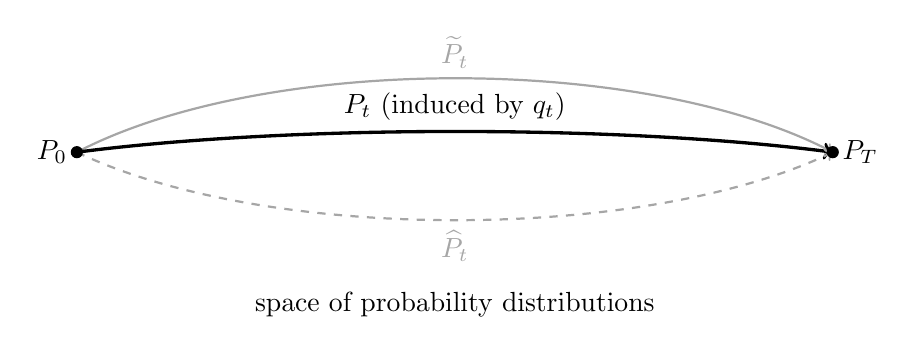
\begin{tikzpicture}[x=1cm,y=1cm]
    \coordinate (P0) at (0,0);
    \coordinate (PT) at (9.6,0);
    \draw[gray!70,thick,->]
      (P0) .. controls (2.4,1.25) and (7.2,1.25) ..
      node[pos=0.5,above,gray!70] {\(\widetilde P_t\)} (PT);
    \draw[black,very thick,->]
      (P0) .. controls (2.7,0.35) and (6.9,0.35) ..
      node[pos=0.5,above] {\(P_t\) (induced by \(q_t\))} (PT);
    \draw[gray!70,thick,dashed,->]
      (P0) .. controls (2.4,-1.15) and (7.2,-1.15) ..
      node[pos=0.5,below,gray!70] {\(\widehat P_t\)} (PT);
    \fill (P0) circle (2.2pt);
    \fill (PT) circle (2.2pt);
    \node[left] at (P0) {\(P_0\)};
    \node[right] at (PT) {\(P_T\)};
    \node[below] at (4.8,-1.65) {space of probability distributions};
\end{tikzpicture}
\end{center}
The kernel \(q_t\) in Eq.~\eqref{eq:forward-perturbed-marginal} determines
the black path \(P_t\). DSM does not choose the path. Once \(q_t\) has been chosen,
DSM draws pairs \(\vct{x}_0\sim P_0\) and
\(\vct{x}_t\sim q_t(\cdot\mid\vct{x}_0)\) and learns the known vector
\(\nabla_{\vct{x}_t}\ln q_t(\vct{x}_t\mid\vct{x}_0)\). Averaging that
vector over the possible starting points at fixed \(\vct{x}_t\) gives
\(\nabla_{\vct{x}_t}\ln P_t(\vct{x}_t)\), as shown in
Eq.~\eqref{eq:conditional-score-identity}. The controlled perturbation therefore
makes this spatial derivative learnable from samples; DSM is not taking a finite
difference between distributions.

It is useful to say that the family \(\{\vct{s}_t\}\) records the chosen path,
with one qualification. At each time,
\(\vct{s}_t=\nabla\ln P_t\) records the local shape of \(P_t\); where the
density is positive on a connected region, it determines \(P_t\) up to the
constant fixed by normalization. But \(\vct{s}_t\) is a spatial derivative,
not the tangent \(\partial_tP_t\) to the curve of distributions, so it does not
by itself say how probability moves in time. A time-dependent velocity field
\(\vct{v}_t\), together with \(P_0\), defines such motion through
\begin{equation*}
    \partial_tP_t+\nabla\cdot(P_t\vct{v}_t)=0.
\end{equation*}
The reverse statement is generally not unique: the same curve \(P_t\) can be
produced by different velocity fields. Thus the drift or probability current
carries the time evolution, while the score describes the distributions visited
along it.

If only the two endpoints and a reference diffusion are specified, the
Schrödinger-bridge problem provides a principled way to choose a connection.
Among all random processes with the required endpoint distributions, it selects
the one with the smallest path-space KL divergence from the reference process---in
plain terms, the stochastic connection requiring the least change to that
reference. Ordinary DSM starts from an already chosen \(q_t\); a
Schrödinger bridge instead makes the connecting process part of the problem
\cite{debortoli2021}.
\end{mdframed}

Expanding the square and averaging first over all possible
\(\vct{x}_0\) at each fixed \(\vct{x}_t\) gives
\begin{equation}
    \mathcal{L}_{\mathrm{DSM}}(t)
    =\mathcal{L}_{\mathrm{SM}}(t)+C_t^{\mathrm{DSM}},
    \label{eq:dsm-sm-equivalence}
\end{equation}
where \(C_t^{\mathrm{DSM}}\) is independent of \(\theta\). For the Gaussian
transition
\begin{equation}
    q_t(\vct{x}_t\mid\vct{x}_0)
    =\mathcal{N}(a_t\vct{x}_0,\nu_t^2 I_d),
    \qquad
    \nabla_{\vct{x}_t}\ln q_t
    =-\frac{\vct{x}_t-a_t\vct{x}_0}{\nu_t^2},
    \label{eq:gaussian-conditional-score}
\end{equation}
so the target is available without differentiating the score network with
respect to its input. DSM is therefore especially convenient for the linear
Gaussian forward diffusions used in most diffusion models. At time \(t\), the
network learns \(\nabla_{\vct{x}_t}\ln P_t(\vct{x}_t)\), the gradient of the
log density of the noisy samples, rather than the corresponding gradient for
the original data density \(P_0\). The latter is recovered only in a regular
zero-noise limit. If \(\nabla_{\vct{x}_t}\ln q_t\) is not available, the usual
computational advantage of DSM is lost.

\subsection{Sliced and implicit sliced score matching}

Sliced score matching probes the score error only along random directions.
Let \(\vct{v}\) be independent of \(\vct{x}\), with
\(M=\mathbb{E}[\vct{v}\vct{v}^{\mathsf{T}}]\) positive definite. Its explicit
form is
\begin{align}
    \mathcal{L}_{\mathrm{SSM}}(t)
    &=\frac{1}{2}\mathbb{E}_{P_t,\vct{v}}\!\left[
      \bigl(\vct{v}^{\mathsf{T}}
      (\vct{s}_{\theta}-\vct{s}_t)\bigr)^2\right]
    \nonumber\\
    &=\frac{1}{2}\mathbb{E}_{P_t}\!\left[
      (\vct{s}_{\theta}-\vct{s}_t)^{\mathsf{T}}
      M(\vct{s}_{\theta}-\vct{s}_t)\right].
    \label{eq:explicit-sliced-score-matching}
\end{align}
If \(M=cI_d\), this is exactly \(c\mathcal{L}_{\mathrm{SM}}(t)\). A general
positive-definite \(M\) gives a different metric but still has
\(\vct{s}_{\theta}=\vct{s}_t\) as its unique unrestricted population optimum.
With a restricted model class, a non-isotropic \(M\) can instead select a
different best approximation.

For the implicit sliced form, define the score Jacobian by
\((J_{\theta})_{ij}=\partial_{x_j}s_{\theta,i}\). Applying integration by parts
along \(\vct{v}\) gives
\begin{equation}
    \mathcal{L}_{\mathrm{SSM}}(t)
    =\underbrace{\mathbb{E}_{P_t,\vct{v}}\!\left[
      \vct{v}^{\mathsf{T}}J_{\theta}\vct{v}
      +\frac{1}{2}(\vct{v}^{\mathsf{T}}\vct{s}_{\theta})^2
      \right]}_{\mathcal{L}_{\mathrm{ISSM}}(t)}+C_{t,M},
    \label{eq:implicit-sliced-score-matching}
\end{equation}
under the same type of boundary assumptions as
Eq.~\eqref{eq:score-matching-integration-by-parts}. When
\(\mathbb{E}[\vct{v}\vct{v}^{\mathsf{T}}]=I_d\), the Hutchinson trace
identity and the same second-moment calculation give~\cite{hutchinson1990}
\begin{equation}
    \mathbb{E}_{\vct{v}}[\vct{v}^{\mathsf{T}}J_{\theta}\vct{v}]
    =\operatorname{tr}J_{\theta},
    \qquad
    \mathbb{E}_{\vct{v}}
      [(\vct{v}^{\mathsf{T}}\vct{s}_{\theta})^2]
    =\lVert\vct{s}_{\theta}\rVert^2.
    \label{eq:sliced-hutchinson-identities}
\end{equation}
Hence the expected implicit sliced loss equals the implicit score-matching
loss in Eq.~\eqref{eq:implicit-score-matching}; a finite number of directions
is an unbiased stochastic trace estimate, not the identical sample loss. One
may reduce its variance by averaging the quadratic term analytically,
\begin{equation}
    \mathcal{L}_{\mathrm{ISSM\text{-}VR}}(t)
    =\mathbb{E}_{P_t,\vct{v}}\!\left[
      \vct{v}^{\mathsf{T}}J_{\theta}\vct{v}
      +\frac{1}{2}\lVert\vct{s}_{\theta}\rVert^2\right].
    \label{eq:variance-reduced-implicit-sliced-score-matching}
\end{equation}
Thus implicit sliced score matching replaces an exact divergence by one or a
few Jacobian--vector products. Here ``implicit'' refers to eliminating the
unknown data score by integration by parts. It is distinct from the statement
that \(P_t\) may be an implicit distribution specified only through samples.

\subsection{Physics-informed enforcement of the Fokker--Planck equation}

Here ``physics-informed'' means enforcing the equation that governs the
probability distribution across time. This is distinct from imposing a physical
residual directly on each generated field, as in physics-informed diffusion
models~\cite{bastek2025physics}.

The preceding objectives compare a model with the score at one time slice.
The Fokker--Planck equation additionally constrains how those slices fit
together. Define the scalar operator
\begin{equation}
    \mathcal{F}_t[\vct{r}]
    =-\nabla\cdot\vct{u}-\vct{u}\cdot\vct{r}
     +\frac{\sigma^2}{2}
      \left(\nabla\cdot\vct{r}+\lVert\vct{r}\rVert^2\right).
    \label{eq:log-fp-operator}
\end{equation}
Equation~\eqref{eq:log-fokker-planck} says that
\(\partial_t\ln P_t=\mathcal{F}_t[\vct{s}_t]\). Taking a spatial gradient
gives the score Fokker--Planck equation
\begin{equation}
    \partial_t\vct{s}_t
    =\nabla\mathcal{F}_t[\vct{s}_t].
    \label{eq:score-fokker-planck}
\end{equation}
A score-based PINN regularizer can therefore use the residual below; related
constructions appear in Refs.~\cite{lai2023,hu2024scorebased}:
\begin{equation}
    \vct{\varepsilon}_{\mathrm{FP}}[\vct{s}_{\theta}]
    =\partial_t\vct{s}_{\theta}
     -\nabla\mathcal{F}_t[\vct{s}_{\theta}],
    \qquad
    \mathcal{L}_{\mathrm{FP}}
    =\frac{1}{2}\mathbb{E}_{\substack{t\sim\rho\\
                          \vct{x}\sim\pi_t}}
      \!\left[\left\lVert
      \vct{\varepsilon}_{\mathrm{FP}}[\vct{s}_{\theta}](\vct{x},t)
      \right\rVert^2\right],
    \label{eq:score-fp-pinn-loss}
\end{equation}
where \(\rho\) and \(\pi_t\) specify the collocation distribution. Forward
samples permit \(\pi_t=P_t\), while a broader collocation law can test the PDE
away from the most probable region.
For jump-driven processes the Fokker--Planck--Lévy equation has a different
spatial operator; a fractional score-based PINN extension is given in
Ref.~\cite{hu2024score}. The present note stays with Brownian diffusion.

Alternatively, a density PINN may parameterize a nonnegative
\(P_{\phi}(\vct{x},t)\) and penalize the original Fokker--Planck residual
\begin{equation}
    \varepsilon_{\mathrm{dens}}[P_{\phi}]
    =\partial_t P_{\phi}
     +\nabla\cdot(\vct{u}P_{\phi})
     -\frac{\sigma^2}{2}\nabla^2P_{\phi}.
    \label{eq:density-fp-pinn-residual}
\end{equation}
This form also needs initial or terminal data, boundary conditions, positivity,
and normalization. The score residual avoids representing exponentially small
density values in high dimension, but it removes the spatially constant part
of \(\ln P_t\), and hence does not determine normalization. Moreover, if
\(\vct{s}_{\theta}\) is a free vector field, conservativity is not guaranteed
solely by calling it a score; one can parameterize
\(\vct{s}_{\theta}=\nabla\Phi_{\theta}\) or add a penalty on the antisymmetric
part of \(J_{\theta}\).
Another route rewrites the Fokker--Planck equation as a continuity equation
and represents the evolving distribution by a score-based normalizing flow,
with its velocity matched through mean-field control~\cite{zhou2025simulating}.
This models the transport field more directly than the local residual above.

A typical hybrid objective is
\begin{equation}
    \mathcal{L}_{\mathrm{total}}
    =\mathbb{E}_{t\sim\rho}\!\left[
      \lambda_{\mathrm{SM}}(t)\mathcal{L}_{\mathrm{DSM}}(t)\right]
     +\lambda_{\mathrm{FP}}\mathcal{L}_{\mathrm{FP}}
     +\lambda_{\mathrm{aux}}\mathcal{L}_{\mathrm{aux}},
    \label{eq:hybrid-score-fp-loss}
\end{equation}
where \(\mathcal{L}_{\mathrm{aux}}\) may impose boundary, anchoring, or
conservativity conditions. At the exact population solution, all score-matching
objectives above identify \(\vct{s}_t\) under their respective assumptions, and
that true score has zero Fokker--Planck residual. The converse is not true
without an anchor at one time and suitable boundary and uniqueness conditions:
many PDE solutions can satisfy a zero interior residual. Thus the PINN loss is
not merely another algebraic form of score matching. It is a cross-time
self-consistency constraint and is most naturally used together with a
data-informed score loss. It also requires higher derivatives---including
\(\nabla(\nabla\cdot\vct{s}_{\theta})\)---so its computational and numerical
behavior differs substantially from DSM and from a one-direction sliced
estimator. Sampling subsets of coordinatewise PDE terms provides a complementary
way to reduce the cost of high-dimensional PINN training~\cite{hu2023tackling}.

\begin{thebibliography}{99}

\bibitem{hirono2024}
Y.~Hirono, A.~Tanaka, and K.~Fukushima,
``Understanding Diffusion Models by Feynman's Path Integral,''
\href{https://arxiv.org/abs/2403.11262}{arXiv:2403.11262} (2024).

\bibitem{song2021scorebased}
Y.~Song, J.~Sohl-Dickstein, D.~P.~Kingma, A.~Kumar, S.~Ermon, and B.~Poole,
``Score-Based Generative Modeling through Stochastic Differential Equations,''
in \emph{International Conference on Learning Representations} (2021),
\href{https://openreview.net/forum?id=PxTIG12RRHS}{OpenReview paper page}.

\bibitem{hyvarinen2005}
A.~Hyv\"arinen,
``Estimation of Non-Normalized Statistical Models by Score Matching,''
\emph{Journal of Machine Learning Research} \textbf{6}, 695--709 (2005),
\href{https://www.jmlr.org/papers/v6/hyvarinen05a.html}{JMLR paper page}.

\bibitem{vincent2011}
P.~Vincent,
``A Connection Between Score Matching and Denoising Autoencoders,''
\emph{Neural Computation} \textbf{23}, 1661--1674 (2011),
\href{https://doi.org/10.1162/NECO_a_00142}{doi:10.1162/NECO\_a\_00142}.

\bibitem{song2020}
Y.~Song, S.~Garg, J.~Shi, and S.~Ermon,
``Sliced Score Matching: A Scalable Approach to Density and Score Estimation,''
in \emph{Proceedings of the 35th Conference on Uncertainty in Artificial
Intelligence}, PMLR \textbf{115}, 574--584 (2020),
\href{https://proceedings.mlr.press/v115/song20a.html}{PMLR paper page}.

\bibitem{debortoli2021}
V.~De Bortoli, J.~Thornton, J.~Heng, and A.~Doucet,
``Diffusion Schr\"odinger Bridge with Applications to Score-Based Generative
Modeling,'' in \emph{Advances in Neural Information Processing Systems}
\textbf{34}, 17695--17709 (2021),
\href{https://proceedings.neurips.cc/paper/2021/hash/940392f5f32a7ade1cc201767cf83e31-Abstract.html}{NeurIPS paper page}.

\bibitem{hutchinson1990}
M.~F.~Hutchinson,
``A Stochastic Estimator of the Trace of the Influence Matrix for Laplacian
Smoothing Splines,'' \emph{Communications in Statistics---Simulation and
Computation} \textbf{19}, 433--450 (1990),
\href{https://doi.org/10.1080/03610919008812866}{doi:10.1080/03610919008812866}.

\bibitem{lai2023}
C.-H.~Lai, Y.~Takida, N.~Murata, T.~Uesaka, Y.~Mitsufuji, and S.~Ermon,
``FP-Diffusion: Improving Score-Based Diffusion Models by Enforcing the
Underlying Score Fokker--Planck Equation,'' in \emph{Proceedings of the 40th
International Conference on Machine Learning}, PMLR \textbf{202},
18365--18398 (2023),
\href{https://proceedings.mlr.press/v202/lai23d.html}{PMLR paper page}.

\bibitem{bastek2025physics}
J.-H.~Bastek, W.~Sun, and D.~M.~Kochmann,
``Physics-Informed Diffusion Models,'' in \emph{International Conference on
Learning Representations} (2025),
\href{https://openreview.net/forum?id=tpYeermigp}{OpenReview paper page}.

\bibitem{hu2024scorebased}
Z.~Hu, Z.~Zhang, G.~E.~Karniadakis, and K.~Kawaguchi,
``Score-Based Physics-Informed Neural Networks for High-Dimensional
Fokker--Planck Equations,'' \emph{SIAM Journal on Scientific Computing}
\textbf{47}, C680--C705 (2025),
\href{https://doi.org/10.1137/24M1638768}{doi:10.1137/24M1638768}.

\bibitem{hu2024score}
Z.~Hu, Z.~Zhang, G.~E.~Karniadakis, and K.~Kawaguchi,
``Score-fPINN: Fractional Score-Based Physics-Informed Neural Networks for
High-Dimensional Fokker--Planck--Lévy Equations,''
\emph{Communications in Computational Physics} \textbf{40}, 1--26 (2026),
\href{https://doi.org/10.4208/cicp.OA-2024-0201}{doi:10.4208/cicp.OA-2024-0201}.

\bibitem{zhou2025simulating}
M.~Zhou, S.~Osher, and W.~Li,
``Simulating Fokker--Planck Equations via Mean Field Control of Score-Based
Normalizing Flows,'' \href{https://arxiv.org/abs/2506.05723}{arXiv:2506.05723}
(2025).

\bibitem{hu2023tackling}
Z.~Hu, K.~Shukla, G.~E.~Karniadakis, and K.~Kawaguchi,
``Tackling the Curse of Dimensionality with Physics-Informed Neural Networks,''
\href{https://arxiv.org/abs/2307.12306}{arXiv:2307.12306} (2023).

\end{thebibliography}

\end{document}
